\documentclass{beamer}

\usepackage[utf8]{inputenc}
\usecolortheme{beaver}
\usepackage{caption}
\usepackage{subcaption}
\usepackage{mathtools}
\usepackage{todonotes}
\usepackage{amsmath}
\usepackage{bm}
\usepackage{listings}
\usepackage{ragged2e}
\usepackage{titlecaps}
\usepackage{fancyvrb}
\usepackage{diagbox}
\usepackage{listings}

\def\ci{\perp\!\!\!\!\!\perp}

\newtheorem{proposition}{Proposition}
\Addlcwords{for a is but and with of in as the etc on to if}

\setbeamertemplate{section in toc}{\inserttocsectionnumber.~\inserttocsection}
\usetheme{Boadilla}
% \makeatletter
% \setbeamertemplate{footline}{%
%     \leavevmode%
%     \hbox{%
%         \begin{beamercolorbox}[wd=.3\paperwidth,ht=2.25ex,dp=1ex,center]{author in head/foot}%
%             \usebeamerfont{author in head/foot}\insertshortauthor\expandafter\beamer@ifempty\expandafter{\beamer@shortinstitute}{}{~~(\insertshortinstitute)}
%         \end{beamercolorbox}%
%         \begin{beamercolorbox}[wd=.55\paperwidth,ht=2.25ex,dp=1ex,center]{title in head/foot}%
%             \usebeamerfont{title in head/foot}\insertshorttitle
%         \end{beamercolorbox}%
%         \begin{beamercolorbox}[wd=.15\paperwidth,ht=2.25ex,dp=1ex,right]{date in head/foot}%
%             \usebeamerfont{date in head/foot}\insertshortdate{}\hspace*{2em}
%             \insertframenumber{} / \inserttotalframenumber\hspace*{2ex} 
%         \end{beamercolorbox}}%
%         \vskip0pt%
%     }
% \makeatother


\title[]{Enhancing and Promoting Data Simulation Capabilities of pgmpy}
\author{Ankur Ankan}
\institute[iCIS, Radboud University]{Institute for Computing and Information Sciences \\ Radboud University}
\date{May 8, 2024}
\begin{document}

\maketitle

\begin{frame}{Applications of Bayesian Networks}
	\begin{minipage}{\textwidth}
		\centerline{pgmpy is a Python package for Bayesian Networks(BNs) and related models.}
	\end{minipage}
	\vspace{2em}
	\begin{columns}
		\begin{column}{0.6\textwidth}
			\begin{itemize}
			\setlength\itemsep{1em}
				\item \textbf{Predictive Modelling:} E.g., predict the ``Income'' given other attributes.
					% \begin{itemize}
					% 	\item Generative model for efficient representation and computation on joint distributions.
					% 	\item Graphical structure adds interpretability.
					% \end{itemize}
				\item \textbf{Causal Inference:} E.g., study gender pay gap.
					% \begin{itemize}
					% 	\item Edges inferred as causal relationship.
					% 	\item Used for causal effect estimation.
					% \end{itemize}
			\end{itemize}
		\end{column}		
		\begin{column}{0.45 \textwidth}
			\begin{figure}
				\centering
				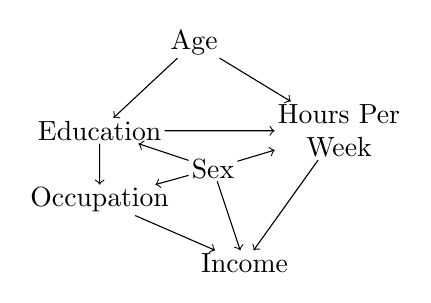
\begin{tikzpicture}[scale=0.8]
				\tikzstyle{every node}=[align=center, inner sep=1pt]
					\node (sex) at (0, -2) {Sex};
					\node (age) at (-0.3, 0) {Age};
					\node (ed) at (-1.8, -1.4) {Education};
					\node (occ) at (-1.8, -2.5) {Occupation};
					\node (hrpw) at (2, -1.4) {Hours Per \\ Week};
					\node (income) at (0.5, -3.5) {Income};
				
					\draw[->]  (age) to (ed);
					\draw[->]  (sex) to (ed);
					\draw[->]  (age) to (hrpw);
					\draw[->]  (ed) to (hrpw);
					\draw[->]  (sex) to (hrpw);
					% \draw[->]  (ed) to (income);
					\draw[->]  (hrpw) to (income);
					\draw[->]  (occ) to (income);
					\draw[->]  (sex) to (income);
					\draw[->]  (ed) to (occ);
					\draw[->]  (sex) to (occ);	
				\end{tikzpicture}
				\caption{\footnotesize{Example of a BN based on Adult Income Dataset [1]}}
			\end{figure}
		\end{column}
	\end{columns}
	\footnotetext[1]{Becker,Barry and Kohavi,Ronny. (1996). Adult. UCI Machine Learning Repository.}
\end{frame}

% \begin{frame}{Applications of Bayesian Networks}
% 	\begin{figure}
% 		\centering
% 		\begin{tikzpicture}
% 			\node at (0, 1)  {
\includegraphics[scale=0.3]{imgs/citation_1.png}};
% 			\node at (4, 0.5)  {
\includegraphics[scale=0.3]{imgs/citation_2.png}};
% 			\node at (0, 0) {
\includegraphics[scale=0.3]{imgs/citation_9.png}};
% 			\node at (5, -0.5) {
\includegraphics[scale=0.3]{imgs/citation_4.png}};
% 			\node at (0, -1) {
\includegraphics[scale=0.3]{imgs/citation_5.png}};
% 			\node at (5, -1.5) {
\includegraphics[scale=0.3]{imgs/citation_6.png}};
% 			\node at (0, -2) {
\includegraphics[scale=0.3]{imgs/citation_7.png}};
% 			\node at (5, -2.5) {
\includegraphics[scale=0.3]{imgs/citation_8.png}};
% 			\node at (0, -3.2) {
\includegraphics[scale=0.3]{imgs/citation_3.png}};
% 		\end{tikzpicture}
% 	\end{figure}
% \end{frame}

\begin{frame}{Simulations in Bayesian Networks}
	Use cases for simulations:
	\vspace{2em}
	\begin{itemize}
		\setlength\itemsep{1em}
		\item \textbf{Approximate Inference:} When exact inference is intractable.
		\item \textbf{Validating Analysis:} Use data from a known model to check if analysis gives correct results.
		\item \textbf{Benchmarking Methods:} Understanding the behavior of new algorithms and methods.
		\item \textbf{Teaching:} Generate data with specific properties to explain various concepts.
	\end{itemize}
\end{frame}

\begin{frame}{Simulation Features in pgmpy}
	Has extensive features for simulation:
	\begin{itemize}
		\item Supports both normal and time-series.
		\item Can specify certain/uncertain/time-series evidence and interventions.
		\item Incorporate other simulation methods.
		\item Optimized implementation.
	\end{itemize}

	% \vspace{1em}
	% \begin{itemize}
	% 	\item No other python package has such extensive simulation features. DagSim comes close.
	% \end{itemize}
	% \todo[inline]{List some other packages here}

	\vspace{2em}
	\centerline{\textcolor{red}{Limited to discrete variables only.}}
	\vspace{2em}
	\begin{itemize}
		\item Adding continuous variable support would significantly increase applicability.
		\item One of the most requested features.
	\end{itemize}

	% Allows simulation from these BNs under various conditions such as
	% (uncertain) evidence, (uncertain) intervention, time-series data,
	% partial simulations for incorporating other simulations.

	% Wide range of features but is limited to discrete variable.

	% Extending this to continuous variables would have a huge impact as it
	% would allow for  a lot of different simulations. No other Python
	% package that offers so much functionality.
\end{frame}

\begin{frame}[fragile]{Fellowship Plan: Phase 1}
	\begin{minipage}{\textwidth}
		\begin{itemize}
			\item Extend simulation capabilities to continuous and mixed variables.
			\item Each node is a BN is parameterized by its conditional distribution given it's parents.
			\item Allow users to specify it in functional form.
		\end{itemize}
	\end{minipage}

	\vspace{2em}
	\begin{columns}
		\begin{column}{0.6\textwidth}
		\begin{figure}
		\begin{tikzpicture}
			\node at (0, 0) {\tiny
				\begin{tabular}{| c | c | c | c | c | c |}
					\hline
					Occu. & \multicolumn{4}{c|}{Teacher} & $ \cdots $ \\
					\hline
					HrPW &  \multicolumn{2}{c|}{$ < 30$} &  \multicolumn{2}{c|}{$\geq 30$} & $ \cdots $ \\
					\hline
					\diagbox[width=2cm]{Income}{Sex} & M & F & M & F & $ \cdots $ \\
					\hline
					High & $ 0.6 $ & $ 0.4 $ & $ 0.55 $ & $ 0.45 $ & $ \cdots $ \\
					\hline
					Low & $ 0.4 $ & $ 0.6 $ & $ 0.45 $ & $ 0.55 $ & $ \cdots $ \\
					\hline
				\end{tabular}
			};
			\draw[double, ->] (0, -1) to (0, -1.5);
			\node at (0, -2) {
					\begin{lstlisting}[basicstyle=\tiny]
function(Income, Occu, HrPW, Sex):
    Occu = DummyEncode(Occu)
    return Gaussian(0.2 * Occ + 0.8 * HrPW + 0.05 * Sex, 1)
				\end{lstlisting}
				};
		\end{tikzpicture}
		\end{figure}
		\end{column}
		\begin{column}{0.4\textwidth}
			\vspace{-5em}
			\begin{figure}
				\centering
				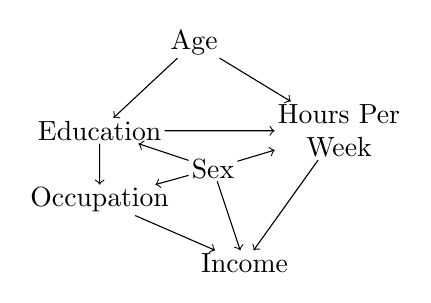
\begin{tikzpicture}[scale=0.8]
				\tikzstyle{every node}=[align=center, inner sep=1pt]
					\node (sex) at (0, -2) {Sex};
					\node (age) at (-0.3, 0) {Age};
					\node (ed) at (-1.8, -1.4) {Education};
					\node (occ) at (-1.8, -2.5) {Occupation};
					\node (hrpw) at (2, -1.4) {Hours Per \\ Week};
					\node (income) at (0.5, -3.5) {Income};

					\draw[->]  (age) to (ed);
					\draw[->]  (sex) to (ed);
					\draw[->]  (age) to (hrpw);
					\draw[->]  (ed) to (hrpw);
					\draw[->]  (sex) to (hrpw);
					% \draw[->]  (ed) to (income);
					\draw[->]  (hrpw) to (income);
					\draw[->]  (occ) to (income);
					\draw[->]  (sex) to (income);
					\draw[->]  (ed) to (occ);
					\draw[->]  (sex) to (occ);	
				\end{tikzpicture}
			\end{figure}
		\end{column}
	\end{columns}
\end{frame}

\begin{frame}{Fellowship Plan: Phase 2}
	Develop tutorials under two user personas:

	\vspace{2em}

	\begin{itemize}
		\item \textbf{Predictive Modelling User:} Focus on approximate inference features, such as specifying different evidences.
		\vspace{1em}
		\item \textbf{Causal Inference User:} Highlighting causal inference features such as simulating data under confounding, interventions, and specifying different types of biases.
	\end{itemize}
\end{frame}

\begin{frame}{Why am I Suitable?}
	\begin{itemize}
		\item Started and maintain the ``pgmpy'' package.
		\item Understand the user base. 
		\item Extensively use simulations in my own research.
	\end{itemize}
\end{frame}

\begin{frame}
	\huge{Thank you.}
\end{frame}
\end{document}
